\paragraph{QuizziPedia::Front-End::Models::MenuBarModel}
		
		\label{QuizziPedia::Front-End::Models::MenuBarModel}
		
		\begin{figure}[ht]
			\centering
			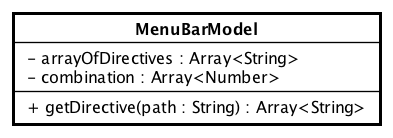
\includegraphics[scale=0.5,keepaspectratio]{UML/Classi/Front-End/QuizziPedia_Front-end_Models_MenuBarModel.png}
			\caption{QuizziPedia::Front-End::Models::MenuBarModel}
		\end{figure} \FloatBarrier
		
		\begin{itemize}
			\item \textbf{Descrizione}: questa classe racchiude i dati necessari per la creazione dinamica della barra menù posizionata in modo fisso su ogni pagina;
			\item \textbf{Utilizzo}: viene utilizzata per memorizzare i dati necessari per la creazione dinamica della barra menù posizionata in modo fisso su ogni pagina;
			\item \textbf{Relazioni con altre classi}: 
			\begin{itemize}
				\item \textbf{IN} \texttt{MenuBarController}: questa classe permette di gestire il menù fisso per ogni pagina;
			\end{itemize}
			\item \textbf{Attributi}: 
			\begin{itemize}
				\item \texttt{- arrayOfDirectives: Array<String>}\\
				Questo attributo contiene l'array di direttive possibili per la creazione dinamica della barra menù posizionata in modo fisso su ogni pagina;
			\end{itemize}
			\begin{itemize}
				\item \texttt{- combination: Array<Number>}\\
				Questo attributo contiene l'array delle combinazioni delle direttive a seconda dell'autore loggato;
			\end{itemize}
			\item \textbf{Metodi}: 
			\begin{itemize}
				\item \texttt{+ getDirective(path: String): Array<String>} \\
				Metodo \textit{getter\ped{G}} che restituisce un array di \texttt{String} contenente le giuste direttive per quella pagina;
			\end{itemize}
		\end{itemize}		
		
		
		